\section{Calculo vectorial en $\mathbb{R}^n$}
\begin{observación}[Recuerdo de algunas definiciones]
    \vspace{-1cm}
    \begin{enumerate}
        \item Norma euclídea en $\mathbb{R}^n$: $\|x\| = \left( \sum_{i=1}^n x_i^2 \right)^{1/2}$ para $x = (x_1, x_2, \ldots, x_n) \in \mathbb{R}^n$.
        \item Distancia euclídea en $\mathbb{R}^n$: $d(x,y) = \|x - y\|$ para $x, y \in \mathbb{R}^n$.
        \item Norma infinita en $\mathbb{R}^n$: $\|x\|_\infty = \max\{|x_1|, |x_2|, \ldots, |x_n|\}$ para $x = (x_1, x_2, \ldots, x_n) \in \mathbb{R}^n$.
        \item Función norma en $\mathbb{R}^n$: Sea $f: \mathbb{R}^n \to \mathbb{R}$ dada por $f(x) = \|x\|$. Entonces, $f$ es continua en $\mathbb{R}^n$.
        \item Conjunto de funciones continuas: Sea $\mathcal{C}(X, \mathbb{R}^n)$ el conjunto de funciones continuas de un espacio topológico $X$ en $\mathbb{R}^n$.
        \item Conjunto de funciones continuas y acotadas: Sea $\mathcal{BC}(X, \mathbb{R}^n)$ el conjunto de funciones continuas y acotadas de un espacio topológico $X$ en $\mathbb{R}^n$.
    \end{enumerate}   
\end{observación}
\begin{observación}
    Si $X$ es compacto, entonces 
    $\mathcal{BC}(X, \mathbb{R}^n) = \mathcal{C}(X, \mathbb{R}^n)$, ya que toda función continua en un espacio compacto es acotada (Teorema de Weierstrass).
\end{observación}
%% Definición polinómica de un hiperplano
\begin{definición}[Hiperplano]
    Un hiperplano en $\mathbb{R}^n$ es un conjunto $H \subset \mathbb{R}^n$ de puntos que satisfacen que
    $$H = \{x \in \mathbb{R}^n : a_1x_1 + a_2 x_2 + \ldots + a_n x_n = b\}$$
    donde $a = (a_1, a_2, \ldots, a_n) \in \mathbb{R}^n \setminus \{0\}$ y $b \in \mathbb{R}$ - constante. \\
    Como consecuencia, un hiperplano tiene un gradiente constante. 
\end{definición}
\begin{definición}[Hipersuperficie]
    Una hipersuperficie en $\mathbb{R}^n$ es un conjunto $S \subset \mathbb{R}^n$ tal que para cada punto $p \in S$ existe un entorno abierto $U \subset \mathbb{R}^n$ de $p$ y un hiperplano $H$ en $\mathbb{R}^n$ tales que $S \cap U$ es homeomorfo a $H$. \\\\
    En otras palabras, es un objeto que tiene una dimensión menor, es suave y localmente parece un plano, aunque globalmente puede estar curvado. 
\end{definición}
\begin{definición}[Parametrización]
    Una parametrización de un conjunto $S \subset \mathbb{R}^n$ es una función continua $\xi: X \subset \mathbb{R}^m \to \mathbb{R}^n$ tal que $\xi(X) = S$. Si $X \subset X^{\prime}$ y $\xi \in \mathcal{C}^1(X, \mathbb{R}^n)$ decimos que la parametrización es de clase $\mathcal{C}^1$. Si $\xi$ es inyectiva, decimos que la parametrización es un homeomorfismo entre $X$ y $S$.
\end{definición}
\begin{definición}[Hipersuperficie parametrizada]
    Una hipersuperficie parametrizada de $\mathbb{R}^n$ es un par $(\xi, S)$ donde la parametrización $\xi: X \subset \mathbb{R}^{n-1} \to \mathbb{R}^n$ es una función continua, con dominio $X \subset \mathbb{R}^{n-1}$ tal que $X$ es conexo (esto garantiza que la hipersuperfice no sea fragmentada) y tal que $S = \xi(X)$. \\
    Diremos que la hipersuperficie es de clase $\mathcal{C}^1$ si la parametrización $\xi$ es de clase $\mathcal{C}^1$.
 \end{definición}
\begin{definición}[Hipersuperficie (parametrizada) de clase $\mathcal{C}^1$]
    Una hipersuperficie parametrizada $(S, \xi) $ se dice de clase $\mathcal{C}^1$ si existe un conjunto abierto $X' \subset \mathbb{R}^{n-1}$ tal que $X \subset X^{\prime}$ y $\xi$ se puede extender a una función de clase $\mathcal{C}^1$ en todo $X^{\prime}$.
\end{definición}
\begin{definición}[Hipersuperficie simple]
    Una hipersuperficie simple es una hipersuperficie parametrizada $(\xi, S)$ en la que si $\xi$ es inyectiva en $X^{\circ}$. 
\end{definición}
\begin{definición}[Vector normal]
    Dada una hipersuperficie parametrizada $(\xi, S)$ de clase $\mathcal{C}^1$, el vector normal en un punto $p = \xi(u) \in S$ es el vector
    $$N_{\xi} = \frac{\partial \xi}{\partial e_1}(u) \times \frac{\partial \xi}{\partial e_2}(u) \times \cdots \times \frac{\partial \xi}{\partial e_{n-1}}(u),$$
    Tomando que $\xi^{\prime} \in \mathcal{M}_{n \times (n-1)}(\mathbb{R})$ es la matriz jacobiana de $\xi$ de tamaño $n \times n-1$ y que $\xi^{\prime}_{[k]} \in \mathcal{M}_{n-1}(\mathbb{R})$ es la matriz jacobiana quitandole la fila $k$-ésima (i.e. es de tamaño $(n-1) \times (n-1)$), entonces el vector normal se puede expresar como
    $$N_{\xi} = \sum_{k = 1}^{n} (-1)^{k+1} \det(\xi^{\prime}_{[k]}) e_k,$$
    donde $\{e_1, e_2, \ldots, e_n\}$ es la base canónica de $\mathbb{R}^n$. \\
    Denotaremos al vector normal unitario por $\hat{N_{\xi}} = \frac{N_{\xi}}{\|N_{\xi}\|}$.
\end{definición}
\ejemplo{
    Sea una parametrización de una esfera en $\mathbb{R}^3$ dada por
    $$\xi(\theta, \phi) = (\sin(\phi)\cos(\theta), \sin(\phi)\sin(\theta), \cos(\phi))$$
    Calculemos las derivadas parciales: 
    $$\frac{\partial \xi}{\partial \theta} = (-\sin(\phi)\sin(\theta), \sin(\phi)\cos(\theta), 0)$$
    $$\frac{\partial \xi}{\partial \phi} = (\cos(\phi)\cos(\theta), \cos(\phi)\sin(\theta), -\sin(\phi))$$
    Entonces la matriz jacobiana es de la forma:
    $$J_{\xi} = \begin{pmatrix}
        -\sin(\phi)\sin(\theta) & \cos(\phi)\cos(\theta) \\
        \sin(\phi)\cos(\theta) & \cos(\phi)\sin(\theta) \\
        0 & -\sin(\phi) \end{pmatrix}$$   

    Ahora, calculamos el vector normal:
    $$N_{\xi} = \sum_{k=1}^{3} (-1)^{k+1} \det(J_{\xi [k]}) e_k = $$ $$= e_1 \begin{vmatrix}
        \sin(\phi)\cos(\theta) & \cos(\phi)\sin(\theta) \\
        0 & -\sin(\phi) \end{vmatrix} - e_2 \begin{vmatrix}
        -\sin(\phi)\sin(\theta) & \cos(\phi)\cos(\theta) \\
        0 & -\sin(\phi) \end{vmatrix} + e_3 \begin{vmatrix}
        -\sin(\phi)\sin(\theta) & \cos(\phi)\cos(\theta) \\
        \sin(\phi)\cos(\theta) & \cos(\phi)\sin(\theta) \end{vmatrix}.$$
    Calculando los determinantes:
    $$ = -\sin^2(\phi)\cos(\theta) e_1 - \sin^2(\phi)\sin(\theta) e_2 - \sin(\phi)\cos(\phi) e_3.$$
}
\begin{proposición}[Propiedades del vector normal]
    Dada una hipersuperficie parametrizada $(\xi, S)$ de clase $\mathcal{C}^1$ con $\xi: X \subset \mathbb{R}^{n-1} \to \mathbb{R}^n$, el vector normal $N_{\xi}$ satisface las siguientes propiedades:
    \begin{enumerate}
        \item[(I)] Para $n = 3$, $N_{\xi} = \partial_1 \xi \times \partial_2 \xi$.
        \item[(II)] $\langle v, N_{\xi} \rangle = |v| \xi^{\prime}$ para todo $v \in \mathbb{R}^n$.
        \item[(III)] $|N_{\xi}| \xi^{\prime}| = \|N_{\xi}\|^2$.
        \item[(IV)] $N_{\xi} \perp \partial_k \xi$ para todo $k = 1, \ldots, n$.
        \item[(V)] $\|N_{\xi}\|$ coincide con el volumen del paralelepípedo formado por los vectores $\partial_1 \xi, \ldots, \partial_n \xi$.
        \item[(VI)] Dada una base del hiperplano ortogonal a $N_{\xi}$, y para cada $k = 1, \ldots, n-1$, $v_k$ el vector que se obtiene al proyectar $\partial_k \xi$ sobre dicho hiperplano expresado en términos de la base escogida, se tiene que
        $$\|N_{\xi}\| = |\det(v_1 | \cdots | v_{n-1})|.$$
    \end{enumerate}
\end{proposición}
\begin{proof}
    \textbf{(I)} Para $n = 3$, tenemos que $\xi: X \subset \mathbb{R}^2 \to \mathbb{R}^3$. La matriz jacobiana es
    $$\xi^{\prime} = \begin{pmatrix}
        \frac{\partial \xi_1}{\partial e_1} & \frac{\partial \xi_1}{\partial e_2} \\
        \frac{\partial \xi_2}{\partial e_1} & \frac{\partial \xi_2}{\partial e_2} \\
        \frac{\partial \xi_3}{\partial e_1} & \frac{\partial \xi_3}{\partial e_2}
    \end{pmatrix}.$$
    Quitando la fila $k$-ésima obtenemos matrices $2 \times 2$:
    $$\xi^{\prime}_{[1]} = \begin{pmatrix}
        \frac{\partial \xi_2}{\partial e_1} & \frac{\partial \xi_2}{\partial e_2} \\
        \frac{\partial \xi_3}{\partial e_1} & \frac{\partial \xi_3}{\partial e_2}
    \end{pmatrix}, \quad \xi^{\prime}_{[2]} = \begin{pmatrix}
        \frac{\partial \xi_1}{\partial e_1} & \frac{\partial \xi_1}{\partial e_2} \\
        \frac{\partial \xi_3}{\partial e_1} & \frac{\partial \xi_3}{\partial e_2}
    \end{pmatrix}, \quad \xi^{\prime}_{[3]} = \begin{pmatrix}
        \frac{\partial \xi_1}{\partial e_1} & \frac{\partial \xi_1}{\partial e_2} \\
        \frac{\partial \xi_2}{\partial e_1} & \frac{\partial \xi_2}{\partial e_2}
    \end{pmatrix}.$$
    Por definición del vector normal:
    $$N_{\xi} = \det(\xi^{\prime}_{[1]}) e_1 - \det(\xi^{\prime}_{[2]}) e_2 + \det(\xi^{\prime}_{[3]}) e_3.$$
    Por otro lado, el producto vectorial de $\partial_1 \xi$ y $\partial_2 \xi$ es:
    $$\partial_1 \xi \times \partial_2 \xi = \begin{vmatrix}
        e_1 & e_2 & e_3 \\
        \frac{\partial \xi_1}{\partial e_1} & \frac{\partial \xi_2}{\partial e_1} & \frac{\partial \xi_3}{\partial e_1} \\
        \frac{\partial \xi_1}{\partial e_2} & \frac{\partial \xi_2}{\partial e_2} & \frac{\partial \xi_3}{\partial e_2}
    \end{vmatrix} = \det(\xi^{\prime}_{[1]}) e_1 - \det(\xi^{\prime}_{[2]}) e_2 + \det(\xi^{\prime}_{[3]}) e_3 = N_{\xi}.$$

    \textbf{(II)} Sea $v = \sum_{i=1}^n v_i e_i \in \mathbb{R}^n$. Entonces:
    $$\langle v, N_{\xi} \rangle = \sum_{i=1}^n v_i \langle e_i, N_{\xi} \rangle = \sum_{i=1}^n v_i \cdot (-1)^{i+1} \det(\xi^{\prime}_{[i]}).$$
    Desarrollando el determinante de $\xi^{\prime}$ por la fila adicional que contiene $v$, y considerando que $\xi^{\prime}$ es una matriz $n \times (n-1)$, podemos extenderla a una matriz $n \times n$ añadiendo $v$ como columna adicional. El determinante de esta matriz extendida es precisamente:
    $$\det\begin{pmatrix} \xi^{\prime} & v \end{pmatrix} = \sum_{i=1}^n (-1)^{n+i} v_i \det(\xi^{\prime}_{[i]}).$$
    Ajustando los signos y notando que el determinante de una matriz con columnas linealmente dependientes puede expresarse en términos de productos escalares, obtenemos $\langle v, N_{\xi} \rangle = |v| \xi^{\prime}$.

    \textbf{(III)} Aplicando la propiedad (II) con $v = N_{\xi}$:
    $$\langle N_{\xi}, N_{\xi} \rangle = |N_{\xi}| \xi^{\prime}.$$
    Pero $\langle N_{\xi}, N_{\xi} \rangle = \|N_{\xi}\|^2$, por lo que $|N_{\xi}| \xi^{\prime}| = \|N_{\xi}\|^2$.

    \textbf{(IV)} Para cualquier $k = 1, \ldots, n-1$, el vector $\partial_k \xi$ es una columna de la matriz jacobiana $\xi^{\prime}$. Consideremos:
    $$\langle N_{\xi}, \partial_k \xi \rangle = \sum_{i=1}^n (-1)^{i+1} \det(\xi^{\prime}_{[i]}) \cdot (\partial_k \xi)_i.$$
    Esto es equivalente al desarrollo del determinante de una matriz $n \times n$ construida al agregar la columna $\partial_k \xi$ a $\xi^{\prime}_{[i]}$. Como $\partial_k \xi$ ya es una columna de $\xi^{\prime}$, esta matriz resultante tiene dos columnas iguales, por lo que su determinante es cero. Por tanto:
    $$\langle N_{\xi}, \partial_k \xi \rangle = 0,$$
    lo que significa que $N_{\xi} \perp \partial_k \xi$ para todo $k = 1, \ldots, n-1$.

    \textbf{(V)} El volumen del paralelepípedo formado por los vectores $\partial_1 \xi, \ldots, \partial_{n-1} \xi$ en $\mathbb{R}^n$ está dado por:
    $$\text{Vol} = \sqrt{\det(G)},$$
    donde $G$ es la matriz de Gram $G_{ij} = \langle \partial_i \xi, \partial_j \xi \rangle$. Por otro lado, usando la fórmula de Cauchy-Binet:
    $$\det(G) = \det(\xi^{\prime T} \xi^{\prime}) = \sum_{1 \leq i_1 < \cdots < i_{n-1} \leq n} [\det(\xi^{\prime}_{[i_1, \ldots, i_{n-1}]})]^2,$$
    donde la suma se toma sobre todas las submatrices $(n-1) \times (n-1)$ de $\xi^{\prime}$. En nuestro caso, esta suma se reduce a:
    $$\det(G) = \sum_{k=1}^n [\det(\xi^{\prime}_{[k]})]^2 = \|N_{\xi}\|^2.$$
    Por tanto, $\|N_{\xi}\| = \sqrt{\det(G)}$ coincide con el volumen del paralelepípedo.

    \textbf{(VI)} Sea $\{w_1, \ldots, w_{n-1}\}$ una base ortonormal del hiperplano ortogonal a $N_{\xi}$. Para cada $k = 1, \ldots, n-1$, la proyección de $\partial_k \xi$ sobre este hiperplano es:
    $$v_k = \sum_{j=1}^{n-1} \langle \partial_k \xi, w_j \rangle w_j.$$
    El volumen del paralelepípedo formado por $v_1, \ldots, v_{n-1}$ en el hiperplano es:
    $$|\det(v_1 | \cdots | v_{n-1})| = |\det([\langle \partial_i \xi, w_j \rangle]_{i,j})|.$$
    Como los $v_k$ son las proyecciones de los $\partial_k \xi$ sobre el hiperplano ortogonal a $N_{\xi}$, y $N_{\xi}$ es perpendicular a este hiperplano, tenemos que:
    $$\|\partial_k \xi\|^2 = \|v_k\|^2 + \left(\frac{\langle \partial_k \xi, N_{\xi} \rangle}{\|N_{\xi}\|}\right)^2.$$
    Pero por la propiedad (IV), $\langle \partial_k \xi, N_{\xi} \rangle = 0$, por lo que $\|\partial_k \xi\| = \|v_k\|$. Por tanto:
    $$\|N_{\xi}\| = |\det(v_1 | \cdots | v_{n-1})|.$$
\end{proof}
\subsection{Concepto de orientación}
\begin{definición}[Preservación de orientación en aplicaciones lineales]
    Dada una aplicación lineal $f: V \to W$ entre dos espacios vectoriales de la misma dimensión y tal que $f$ es invertible (ya que si no, no tiene sentido hablar de orientación ($\det(f) = 0$)). Dada una base $B$ de $V$ y una base $C$ de $W$, definimos la preservación de la orientación de la siguiente manera:
    $$\text{Si } \det([f]_B) > 0 \text{, entonces } f \text{ preserva la orientación},$$
    $$\text{Si } \det([f]_B) < 0 \text{, entonces } f \text{ invierte la orientación}.$$
\end{definición}
\begin{definición}[Preservación de orientación en aplicaciones diferenciables]
    Dada $F: A \subset \mathbb{R}^n \to \mathbb{R}^n$ diferenciable tal que $J_F(x) \neq 0$ para todo $x \in A$, decimos que $F$ preserva la orientación si $\det(J_F(x)) > 0$ para todo $x \in A$ y que invierte la orientación en caso contrario. Equivalentemente si la aplicación diferencial $\partial_x F: \mathbb{R}^n \to \mathbb{R}^n$ está orientada positivamente respecto a las bases canónicas de $\mathbb{R}^n$ para todo $x \in A$.
\end{definición}
\begin{definición}[Orientación de las hipersuperficies compactas]
    Sea $(\xi, S)$ una hipersuperficie parametrizada de clase $\mathcal{C}^1$. Si $S = \partial A$ para algún $A$ $\mathbb{R}^n$-acotado, abierto y conexo, decimos que $(\xi, S)$ está orientada positivamente si $N_{\xi}$ apunta a la cara exterior de $A$.
\end{definición}
\begin{observación}
    Estas dos nociones pueden entrar en conflicto de la siguiente manera: 
    Supongamos que $(\xi, S)$ es una hipersuperficie parametrizada $\mathcal{C}^1$ y que $S= \partial A$ para algun $A \subset \mathbb{R}^n$-acotado, abierto y conexo. \\
    Por definición de vector normal, está escogido de forma que siempre tiene orientación positiva respecto a la base dada por $\xi^{\prime}$, es decir, la matriz $(N_{\xi} | \xi^{\prime})$ tiene determinante positivo. No obstante podría ocurrir que está noción de orientación positiva no concordase con la de las superficies, esto es, que el vector normal apuntase a la cara de dentro de la hipersuperficie y por lo tanto etnga orientacion negativa respecto a la de la superficie.
\end{observación}
\ejemplo{
    En $\mathbb{R}^n$ definmos las coordenadas $(n-1)$-esféricas como el sistema de coordenadas: 
    $$\begin{cases}
        x_1 = r\cos(\phi_1) \\
        x_2 = r\sin(\phi_1)\cos(\phi_2) \\
        x_3 = r\sin(\phi_1)\sin(\phi_2)\cos(\phi_3) \\
        \vdots \\
        x_{n-1} = r \sin(\phi_1)\ldots \sin(\phi_{n-2})\cos(\phi_{n-1}) \\
        x_n = r \sin(\phi_1)\ldots \sin(\phi_{n-2})\sin(\phi_{n-1})
    \end{cases}$$
    done $r \in \mathbb{R}^+$ y $\phi_1, \ldots, \phi_{n-2} \in (0, \pi)$ y $\theta \in (0, 2\pi)$. Obsérvese que estas coordenadas coinciden con las coordenadas polares cuando $n = 2$ y con las esféricas cuando $n = 3$. \\
    Sea $\Delta (r, \phi_1, \ldots, \phi_{n-2}, \theta)$ la transformación asociada a este cambio de variables. La matriz jaobiana del cambio de coordenadas, es decir $J_{\Delta}$ viene dada por: 
    $$J_{\Delta} = \begin{matrix} 
        \frac{\partial x_1}{\partial r} & \frac{\partial x_1}{\partial \phi_1} & \cdots & \frac{\partial x_1}{\partial \theta} \\
        \frac{\partial x_2}{\partial r} & \frac{\partial x_2}{\partial \phi_1} & \cdots & \frac{\partial x_2}{\partial \theta} \\
        \vdots & \vdots & \ddots & \vdots \\
        \frac{\partial x_n}{\partial r} & \frac{\partial x_n}{\partial \phi_1} & \cdots & \frac{\partial x_n}{\partial \theta}
    \end{matrix}$$ 
    Siendo su determinante: 
    $$\det(J_{\Delta}) = r^{n-1} \sin^{n-2}(\phi_1) \sin^{n-3}(\phi_2) \cdots \sin(\phi_{n-2}).$$\\
    Si ahora asumimos que $r = 1$ estamos restringiendonos a la esfera $\mathbb{S}^{n-1}$ por lo que podemos considerar la hipersuperfice parametrizada simple $\mathcal{C}^1$ donde $\xi [0, \pi)^{n-2} \times [0, 2\pi) \to \mathbb{R}^n$ dada por:
    $$\xi(\phi_1, \ldots, \phi_{n-1}) = \Delta(1, \phi_1, \ldots, \phi_{n-1}).$$
    Con esta parametrización, el vector normal de la esfera es: 
    $$N_{\xi}(\phi_1, \ldots, \phi_{n-1}) = \sin^{n-2}(\phi_1) \sin^{n-3}(\phi_2) \cdots \sin(\phi_{n-2}) \xi(\phi_1, \ldots, \phi_{n-2})$$
    Por último observamos que
    $$\int_{[0, \pi)^{n-2}} |J_{\Delta}(1, \phi_1, \ldots, \phi_{n-2}) | d\phi_1 \ldots d\phi_{n-1} = $$
    $$ = \int_{0}^{2\pi} \sin^{n-2}(\phi_1) d\phi_1 \int_{0}^{\pi} \sin^{n-3}(\phi_2) d\phi_2 \cdots \int_{0}^{\pi} \sin(\phi_{n-2}) d\phi_{n-2} = vol(\mathbb{S}^{n-1})$$
    La aplicación $\Delta$ tiene orientación positiva como aplicación diferencial ya que $\Delta^n$ tiene orientación positiva como aplicación lineal dado que $J_{\Delta} > 0$. por otra parte $N_{\xi} = \alpha \xi$ con $\alpha > 0$ , luego 
    $$|N_{\xi}^i| = |\alpha \xi^i| = \alpha|\xi^i| = \alpha^n J_{\Delta} > 0$$
    es decir, la orientación de $|N_{\xi}|(\xi^{i})$ coincide con la de $\Delta$. Además, la orientación de $h$ como hipersuperficie compacta es siempre positiva (coincide con la de $\Delta$ ya que el vector normal $N_{\xi}$ tiene la misma dirección y sentido que el vector de posición $\xi$, que apunta siempre hacia la componente conexa no limitada del complementario de la superficie). 
}
\subsection{Los operadores fundamentales del cálculo vectorial}
\begin{definición}[Gradiente]
    Sea $f: A \subset \mathbb{R}^n \to \mathbb{R}$ una función diferenciable en $A$. El gradiente de $f$ en un punto $x \in A$ es el vector en $\mathbb{R}^n$ definido como
    $$\nabla f(x) = \left( \frac{\partial f}{\partial x_1}(x), \frac{\partial f}{\partial x_2}(x), \ldots, \frac{\partial f}{\partial x_n}(x) \right)$$
\end{definición}
\begin{definición}[Divergencia]
    Sea $F: A \subset \mathbb{R}^n \to \mathbb{R}^n$ una función diferenciable en $A$. La divergencia de $F$ en un punto $x \in A$ es el escalar definido como
    $$\text{div } F(x) = \sum_{i=1}^n \frac{\partial F_i}{\partial x_i}(x) = \nabla \cdot F(x) = \langle \nabla, F(x) \rangle$$
    Básicamente, mide la tasa de cambio neta de un campo vectorial en un punto, es decir, cuánto "flujo" sale o entra en ese punto.
\end{definición}
\begin{definición}[Laplaciano]
    Sea $f: A \subset \mathbb{R}^n \to \mathbb{R}$ una función diferenciable en $A$. El laplaciano de $f$ en un punto $x \in A$ es el escalar definido como
    $$\Delta f(x) = \text{div } (\nabla f(x)) = \sum_{i=1}^n \frac{\partial^2 f}{\partial x_i^2}(x)$$    
\end{definición}
\begin{definición}[Rotacional]
    Sea $F: A \subset \mathbb{R}^3 \to \mathbb{R}^3$ una función diferenciable en $A$. El rotacional de $F$ en un punto $x \in A$ es el vector definido como
    $$\text{rot} F(x) = \nabla \times F(x) = \begin{vmatrix}
        e_1 & e_2 & e_3 \\
        \frac{\partial}{\partial x_1} & \frac{\partial}{\partial x_2} & \frac{\partial}{\partial x_3} \\
        F_1(x) & F_2(x) & F_3(x)
    \end{vmatrix}$$
    Básicamente mide la tendencia de un campo vectorial a rotar alrededor de un punto.
\end{definición}
\begin{proposición}
    Sea $F: A \subset \mathbb{R}^3 \to \mathbb{R}^3$ una función diferenciable en $A$. Entonces, para todo $x \in A$ se cumple que
    $$\text{div}(\text{rot } F)(x) = 0$$
\end{proposición}
\begin{proposición}
    Sea $f: A \subset \mathbb{R}^3 \to \mathbb{R}$ una función diferenciable en $A$. Entonces, para todo $x \in A$ se cumple que
    $$\text{rot}(\nabla f)(x) = 0$$
\end{proposición}
\subsection{Integrales geométricas}
\begin{definición}[Integral de campo vectorial]
    Sea $(\xi, S)$ una hipersuperfice parametrizada $C^1$ con $\xi: X \subset \mathbb{R}^{n-1} \to \mathbb{R}$ y $F \in C(S, \mathbb{R}^n)$. Definimos la integral del campo vectorial $F$ sobre $S$ como 
    $$\int_S F = \int_X \langle F \circ \xi, N_{\xi} \rangle $$
    Sea $f \in C(S, \mathbb{R})$ definimos la integral de campo escalar $f$ sobre $S$ como 
    $$\int_S f = \int_X (f \circ \xi) \|N_{\xi}\|$$
    En el caso particular de que $f \equiv 1$ decimos que $vol(S) = \int_S 1 = \int_X \|N_{\xi}\|$ es la medida (área en el caso de $n = 3$ y volumen en el caso de $n = 4$) de la hipersuperficie $S$.
\end{definición}
\begin{definición}[Integrales de línea]
    Dada $F: A \subset \mathbb{R}^n \to \mathbb{R}^n$ y un camino absolutamente contiuo $\gamma: [a, b] \to A$, denotamos la integral de $F$ a lo largo del camino $\gamma$ como 
    $$\oint_{\gamma} F = \int_a^b \langle F(\gamma(t)), \gamma^{\prime}(t)\rangle dt$$
    Sea $f: A \subset \mathbb{R}^n \to \mathbb{R}$, definimos la integral de un campo escalar $f$ a lo largo del camino $\gamma$ como
    $$\int_{\gamma} f = \int_a^b f(\gamma(t)) \|\gamma^{\prime}(t)\| dt$$
\end{definición}
\begin{observación}
    Como $\gamma = (\gamma_1, \ldots, \gamma_n)$ es absolutamente continua, sus componentes $\gamma_k$ también lo son y por el teorema fundamental del cálculo, las $\gamma_k^{\prime}$ existen en casi todo punto y $\gamma_k^{\prime} \in L^1([a,b], \mathbb{R}^n)$. Si $F \circ \gamma \in L^1([a,b], \mathbb{R}^n)$ entonces $\langle F(\gamma(t)), \gamma^{\prime}(t)\rangle \in L^1([a,b], \mathbb{R})$ por lo que existe $\oint_{\gamma} F$. Un razonamiento similar puede aplicarse a $\oint_{\gamma} f$.
\end{observación}
\begin{observación}
    POr el teorema del cambio de variable, $\oint_{\gamma} F$ y $\oint_{\gamma} f$ no dependen de la parametrización $\gamma(I)$ siempre que la parametrización preserva la orientación del camino. 
\end{observación}
\subsection{Curvas rectificables}
\begin{definición}[Parametrizaciones equivalentes]
    Sean $I, J \subset \mathbb{R}$-intervalos, $(Y, d)$ un espacio métrico y $u: I \to Y, $ y $v: J \to Y$ dos funciones continuas. Diremos que son equivalentes si existen dos aplicaciones monótonas $\varphi: I \to J$ y $\psi: I \to J$ ales que $u(t) = v(\varphi(t)) \forall t \in I$ y Equivalentemente $u(\psi(s)) = v(s) \forall s \in J$. \\
    Denotaremos $u \sim v$ si $u$ y $v$ son equivalentes y a $\varphi$ y $\psi$ las denominamos cambios de parámetro. 
\end{definición}
\begin{observación}
    La relación definida anteriormente es una relación de equivalencia. 
\end{observación}
\begin{definición}[Curva]
    Una cruva $\gamma$ es una clase de equivalencia de representaciones paramétricas. En el caso $Y = \mathbb{R}^n$, se dice que la curva $\gamma$ es $C^n$ si admite una representación de clase $C^n$. \\
    Si $u: [a,b] \to Y$ es una representación paramétrica de $\gamma$ y $u(a) = ub(b)$ entonces $\gamma$ es una curva cerrada. Asimismo, también se define curva simple si $u$ es inyectiva en $[a,b)$.
\end{definición}
\begin{lema}
    Si $u: I \to Y$ es una representación paramétrica de una curva $\gamma$, entonces existe otra representación paramétrica $v: J \to Y$ no constante en intervalos no degenerados. 
\end{lema}
\begin{proof}
    Por simplicidad, asumamos que $I = [a,b]$ es compacto (en el caso general bastaría con particionar adecuadamente $I$ en intervalos compactos). Construiremos una serie de funciones que nos ayudarán a obtener la parametrización buscada: \\
    Comencemos definiendo en $I$ la relación $t \sim s \iff u(\tau) = u(t) = u(s) \forall \tau \in [\min(t,s), \max(t,s)]$ es constante. Dado que esta relación es de equivalencia y que por esr $u$ continua y $I$ compacto, las clases de equivalencia son intervalos compactos.\\
    Sea $g: I \to I$ dada por $g(t) = \max{t}_{\sim} = \max\{s \in I : s \sim t\}$, g es creciente y $u \circ g = u$. \\
    Sea $\psi: I \to \mathbb{R}$ tal que $\psi(x) = \lambda_1(g[a,x)) = \lambda_1(\{g(t) : t \in [a, x)\})$. La función $\psi$ lo que hace es medir el intervalo después de haber contraído todos los puntos en los que la curva era constante, por lo que $\psi$ es creciente y contractiva, ya que dado $y > x$ 
    $$0 \leq \psi(y) - \psi(x) = \lambda_1(g[a,y)\setminus g[a,x))= \lambda_1(g[x,y]) \leq \lambda_1([x,y]) = y - x$$ 
    Por lo tanto $\psi$ es continua y $J = \psi(I)$ es un intervalo. \\
    Definimos entonces el cambio de parámetro $\varphi(t) = \max\{\psi^{-1}(\{t : t \in J\})\}$. Se tiene entonces que $\varphi$ es creciente y $\psi(\varphi(t)) = t$. \\
    Veamos ahora que $v = u \circ \varphi$ no es constante en intervalos no degenerados: Supongamos que $u \circ \varphi$ es constante en $[t, s] \subset J$ Así, $g(\varphi(t)) = g(\varphi(s))$ por lo que
    $$s - t = \psi(\varphi(s)) - \psi(\varphi(t)) = \lambda_1(g[\varphi(t), \varphi(s)]) = 0$$ 
    y por lo tanto $[t, s]$ es degenerado. \\
    Para finalizar, vemos que $u$ es continua: Sea $t_n \to t$ Si $\varphi(t_n) \to \varphi(t)$ entonces $u(\varphi(t_n)) = u(g(\varphi(t_n)))$ y si no $\varphi(t_n) \to x < \varphi(t)$ y $u(x) = u(\varphi(t))$ por lo que $u(\varphi(t_n)) = u(g(\varphi(t_n)))$.
\end{proof} 
\begin{definición}[Longitud de una curva]
    Sea $(Y, d)$ un espacio métrico y $\gamma$ una curva en $Y$. Sea $u: I \to Y$ una representación paramétrica de $\gamma$, donde $I = [a, b] \subset \mathbb{R}$ es un intervalo, entonces definimos la longitud de $\gamma$ como 
    $$L(\gamma) = Var_I(u)  = \sup\{\sum_{k = 1}^{n} d(u(t_k), u(t_{k-1})) : a = t_0, \ldots, t_n = b, n \in \mathbb{N}\}$$  
    $Var_{K}(u)$ se llama variación total de la función $u$. Decimos que la curva $\gamma$ es rectificable si $L(\gamma) < \infty$. \\
    Decimos que $\gamma$ es \textbf{localmente rectificable} si $Var_{[a,b]}(u) < \infty$ para todo intervalo $[a,b] \subset I$ 
\end{definición}
\begin{proposición}
    Sea $(Y, d)$ un espacio métrico. Dadas dos representaciones paramétricas $u: I \to Y$ y $v: J \to Y$ son equivalentes, etnonces $Var_I(u) = Var_J(u)$. En consecuencia, las definiciones de rectificabilidad y de longitud de una curva no dependen de la representación paramétrica particular. 
\end{proposición}
\begin{proposición}
    Sea $I \subset \mathbb{R}$ un intervalo, sea $(Y, d)$ un espacio métrico y sea $u: I \to Y$ una función. Si $c \in I$ entonces
    $$Var_{I \cap (-\infty, c]}(u) + Var_{I \cap [c, +\infty)}(u) = Var_I(u)$$
\end{proposición}
\begin{teorema}
    Sea $Y$ una curva rectificable en $\mathbb{R}^n$ con representación paramétrica $u: I \to \mathbb{R}^n$ donde $I \subset \mathbb{R}$ es un intervalo. Entonces $u^{\prime}$ existe en casi todo punto y se cumple que
    $$\int_I \|u^{\prime}(t) dt\| \leq L(\gamma)$$
    La igualdad se cumple si y sólo si $u \in AC(I; \mathbb{R}^n)$
\end{teorema}
\begin{definición}[Curva parametrizada por longitud de arco]
    Sea $(Y, d)$ un espacio métrico. Dada una curva localmente rectificable $\gamma$ en $Y$, decimos que $\gamma$ está parametrizada por longitud de arco se admite una representación paramétrica $\gamma: J \to Y$ tal que 
    $$Var_{[t,s]}(\gamma) = t - s$$
    para todo $t,s \in J$ con $t < s$ \\
    Intuitivamente, significa que una curva crece a la misma "velocidad" a que se recorre el intervalo que la define. \\
    Equivalentemente a esta definición, una curva $\gamma$ también se puede decir que se puede parametrizar por longitud de arco si existe una representación paramétrica $u: J \to Y$ tal que
    $$\|u^{\prime}(t)\| = 1 \text{ para casi todo } t \in J$$
\end{definición}
\begin{observación}
    Obsérvese que la funciñon $\gamma$ es es lipschitziana cuya constante es menor o igual que 1, ya que 
    $$d(\gamma(t), \gamma(s)) \leq Var_{[s,t]}(\gamma) = |t - s|$$ 
    para todo $t, s \in J : t < s$. 
\end{observación}
\begin{proposición}
    Sea $\gamma$ una curva en $\mathbb{R}^n$. Supongamos que $\gamma$ puede ser parametrizada por longitud de arco y sea $\omega: J \to \mathbb{R}^n$ una representación por longitud de arco. Entonces 
    $$\|\omega^{\prime}(s)\| = 1 \text{ para casi todo } s \in J$$
\end{proposición}
\begin{proof}
    Como $\omega$ es lipschitziana, es absolutamente continua y por tanto derivable para casi todo $s \in J$. Y por una proposición anterior se tiene que 
    $$L(\gamma) = s_2 - s_1 \geq \|\omega(s_2) - \omega(s_1)\| \iff \|\frac{\omega(s_2) - \omega(s_1)}{s_2 - s_1}\| \leq 1$$
    por lo que $\|\omega^{\prime}(s)\| \leq 1$ para $\lambda_1$-casi todo $s \in J$\\
    Por otra parte, se tiene que 
    $$\lambda_1(J_1) = Var_{J_1}(\omega) = \int_{J_1} \|\omega^{\prime}(s)\|ds$$
    Así, se tiene que 

    $$0 = \lambda_1(J_1) - \int_{J_1} \|\omega^{\prime}(s)\|ds = \int_{J_1} (1 - \|\omega^{\prime}(s)\|) ds$$
    Dado que $\|w^{\prime}(s)\| \leq 1$ para casi todo $s \in J_1$, necesariamente $\|\omega^{\prime}\| = 1$ para casi todo $s \in J_1$.
\end{proof}
\begin{teorema}
    Sea $(Y, d)$ un espacio métrico y $\gamma$ una curva continua localmente rectificable. Entonces, $\gamma$ puede ser parametrizada por longitud de arco. 
\end{teorema}
\begin{proof}
    Consideremos una parametrización $u: I \to Y$ de $\gamma$ no constante en intervalos no degenerados y $t_0 \in I$. Puede comprobarse que la función 
    $$V(t) = \begin{cases}
        \text{Var}_{[t_0, t]}(u) & \text{si } t \geq t_0 \\
        -\text{Var}_{[t, t_0]}(u) & \text{si } t < t_0
    \end{cases}$$
    es continua, creciente y sobreyectiva sobre su imagen. Así, $J = V(I)$ es un intervalo. 
    
    Afirmamos que $V$ es estrictamente creciente. Dados $t_1 < t_2$ tales que $V(t_1) = V(t_2)$, entonces o bien $t_1, t_2 \geq t_0$ o bien $t_1, t_2 \leq t_0$, y en ambos casos se tiene que 
    $$\text{Var}_{[t_1, t_2]}(u) = 0$$
    lo que implica que $u$ es constante en el intervalo $[t_1, t_2]$, contradiciendo la hipótesis. 
    
    Por tanto, $V: I \to J$ es un homeomorfismo y admite inversa continua $V^{-1}: J \to I$. Definimos 
    $$\omega(s) = u(V^{-1}(s))$$
    que es la parametrización por longitud de arco buscada, pues para $s_1 < s_2$ en $J$ se tiene
    $$\text{Var}_{[s_1, s_2]}(\omega) = \text{Var}_{[V^{-1}(s_1), V^{-1}(s_2)]}(u) = s_2 - s_1$$
\end{proof}
\begin{teorema}
    Sea $\mathcal{CR}$ el espacio de parametrizaciones $u: [0,1] \to \mathbb{R}^n$ de curvas rectificables en $\mathbb{R}^n$ y consideremos la distancia entre $u$ y $v$ dada por $d(u, v) = \|u -v\|_{\infty} + Var(u-v)$. Entones la función de longitud de arco $L: \mathcal{CR} \to \mathbb{R}$ es una función continua. 
\end{teorema}
\begin{teorema}
    Sea $\gamma$ una curva simple (inyectiva) rectificable en $\mathbb{R}^2$ de longitud $L(\gamma)$. Para cada $h > 0$ denotemos $\gamma_h$ al conjunto de los puntos del plano que están a una distancia no mayor que $h$ de $\gamma$, es decir
    $$\gamma_h = \{x \in \mathbb{R}^2 : \|x - y\| \leq h \text{ para algún } y \in \gamma\}$$
    Entonces 
    $$\lambda_2(\gamma_h) \leq \pi h^2 + 2hL(\gamma)$$
\end{teorema}
\begin{proof}
    Si $\gamma$ es un segmento de la recta, la región $\gamma_h$ es la unión de un rectángulo y de dos discos semicirculares, y en este caso el área de $\gamma_h$ es exactamente igual a $\pi h^2 + 2hL(\gamma)$. \\
    Si $\gamma$ es una curva formada por dos segmentos de recta, el conjunto $\gamma_h$ es la unión de dos rectángulos solapados, dos discos semicirculares y un sector circular. Como el área del sector circular no excede el área al área del cuadrilátero formado por los rectángulos solapados, se deduce que en este caso el área de $\gamma_h$ no excede a $\pi h^2 + 2hL(\gamma)$. \\
    Un argumento similar se puede emplear para demostrar la desigualdad 
    $$\lambda_2(\gamma_h) \leq \pi h^2 + 2hL(\gamma)$$
    para cualquier curva poligonal $\gamma$ utilizando inducción sobre el número de aristas. \\
    Para demostrar el teorema para una curva rectificable arbitraria $\gamma$, dejamos $\delta > 0$ dado y construamos un polígono inscrito $P$ con vértices $p_0, p_1, \ldots, p_n$ tal que todo punto del segmento de $\gamma$ que une $p_{k-1}$ y $p_k$ está a una distancia menor que $\delta$ del segmento de recta entre $p_{k-1}$ y $p_k$. \\
    Si un punto está a una distancia menor o igual que $h$ de $\gamma$, entonces está a una distancia menor que $h + \delta$ de $P$. Por tanto, $\gamma_h \subset P_{h + \delta}$ entonces tenemos 
    $$\lambda_2(\gamma_h) \leq \lambda_2(P_{h + \delta}) \leq \pi (h + \delta)^2 + 2(h + \delta)L(P) \leq \pi(h+ \delta)^2 + 2(h + \delta)L(\gamma)$$
    Pero como $\delta$ es arbitrario, se deduce que se debe tener que 
    $$\lambda_2(\gamma_h) \leq \pi h^2 + 2hL(\gamma)$$
\end{proof}
\begin{teorema}
    Consideremos el espacio $\mathcal{CR}_C$ de parametrización de curvas cerradas rectificables con norma $\|\cdot\|_{\infty}$ entonces la función $A: \mathcal{CR}_C \to \mathbb{R}$ que da el área de la región limitada por la curva es continua. 
\end{teorema}
\begin{proof}
    Sea $\epsilon \in \mathbb{R}^+$ y $u \in \mathcal{CR}_C$ encerrado en la región $B$. Sea $\delta \in \mathbb{R}^+$ tal que $\pi \delta^2 + 2\delta L(u) < \epsilon$ y sea $v \in \mathcal{CR}$ encerrado en la región $C$ tal que $\|u - v\|_{\infty} < \delta$.  Entonces, 
    $$|A(B) - A(C)| \leq \lambda_2(B \Delta C) \leq \pi \delta^2 + 2\delta L(u) < \epsilon$$
    por lo que $A$ es continua. 
\end{proof}
\subsection{Campos gradientes y funcions potenciales}
\begin{definición}[Campo gradiente y función potencial]
    Sea $A \subset \mathbb{R}^n$ abierto, $F \in \mathcal{C}(A, \mathbb{R}^n)$. Decimos que $F$ es un campo gradiente o campo integrable, si existe $f \in \mathcal{C}^1(A, \mathbb{R})$ tal que $F = f^{\prime}$. Se dice que $f$ es una función potencial de $F$. 
\end{definición}
\begin{definición}[Estrellado]
    Un conjunto $X \subset \mathbb{R}^n$ se dice estrellado respecto de $p \in X$ si 
    $$tx + (1 - t)p \in X$$ 
    para todo $t \in [0, 1]$ y $x \in X$.
\end{definición}
\begin{lema}[Lema de Poincaré]
    Sea $A \subset \mathbb{R}^n$ abierto, $F \in \mathcal{C}^1(A, \mathbb{R}^n)$. Si $F$ es un campo gradiente, entonces $F^{\prime}$ es una matriz simétrica, es decir, $\partial_j F_k = \partial_k F_j$ para todo $j, k = 1, \ldots, n$. Además, si $A$ es estrellado respecto de un punto, el recíproco también es cierto. 
\end{lema}
\begin{proof}
    Si $F$ es un gradiente, $F = f^{\prime}$ para algún $f \in \mathcal{C}^2(A, \mathbb{R})$ y por el Teorema de Schwartz, las derivadas parciales cruzadas son iguales, así
    $$\partial_j F_k = \partial_j \partial_k f = \partial_k \partial_j f = \partial_k F_j \iff F^{\prime} \text{ es simétrica}$$
    El recíproco es un caso particular de este lema: \\
    Supongamo, sin pérdida de generalidad, que $A$ es estrellado respecto de $0$, si no, basta obtenerlo a través de una traslación. Tomamos el potencial de forma
    $$W_F(x) = \int_0^1 \langle F(tx), x \rangle dt = \sum_{k = 1}^{n} x_k \int_0^1 F_k(tx) dt $$
    $W_F$ está bien definida ya que $tx \in A$ para todo $x \in A$  y $t \in [0, 1]$ por ser $A$ estrellado respecto de $0$. Así, para $x \in A$ tenemos por una parte, 
    $$F_j(x) = 1 \cdot F_j(x) - F_j(0) \cdot 0 = \int_{0}^{1} \frac{d}{dt}(F_j(tx)) dt = \sum_{k = 1}^{n} x_k \int_{0}^1 \partial_k F_j(tx)dt + \int_{0}^{1} F_j(tx)dt$$
    Por otra parte, 
    $$\partial_j W_F(x) = \int_{k = 1}^{n} x_k \int_0^1 \partial_j F_k(tx) dt + \int_0^1 F_j(tx) dt$$
    Como $\partial_j F_k = \partial_k F_j$ concluímos que $\partial_j W_F(x) = F_j(x)$ para todo $x \in A$
\end{proof}
\begin{observación}
    Podemos interpretarl la proposición anterior en términos físicos. Si $F$ es una fuerza física, la función $W_F$ es el trabajo realizado por dicha fuerza al desplazar el objeto sometido a dicha fuerza de posición $0$ a posición $x$ siguiendo una línea recta. Como el campo es conservativo, se tiene que $W_F^{\prime} = F$.
\end{observación}
\begin{teorema}[Teorema fundamental del cálculo para una integral de línea]
    Sea $\gamma: [a, b] \to \mathbb{R}^n$ una curva absolutamente continua y $A$ un abierto tal que $\gamma([a,b]) \subset A \subset \mathbb{R}^n$ \\
    Si $F: A \to \mathbb{R}^n$ es tal que $F \circ \gamma \in L^1([a, b], \mathbb{R}^n)$ entonces la función $f: [a, b] \to \mathbb{R}$ dada por 
    $$f(x) = c + \oint_{\gamma|_{[a,x]}} F$$
    donde $c \in \mathbb{R}$ es una constante cualquier y es derivable en casi todo punto y $f^{\prime} = \langle F \circ \gamma, \gamma^{\prime} \rangle$ en casi todo punto.\\
    Si $g \in \mathcal{AC}(A, \mathbb{R})$ es tal que $g^{\prime} \circ \gamma \in L^1([a,b], \mathbb{R}^n)$ entonces
    $$g(\gamma(b)) - g(\gamma(a)) = \oint_a^b g^{\prime}$$   
\end{teorema}
\begin{proof}
    Basta aplicar el teorema fundamental del cálclo para la integral de Lebesgue. En efecto: 
    $$f^{\prime}(x) = \frac{d}{dx} \int_a^x \langle F(\gamma(t)), \gamma^{\prime} \rangle dt = \langle F(\gamma(x)), \gamma^{\prime(x) }\rangle$$
    para casi todo $x \in [a, b]$. \\
    Por otra parte, si $g \in \mathcal{AC}(A, \mathbb{R})$ es tal que $g^{\prime} \circ \gamma \in L^1([a,b], \mathbb{R}^n)$, entonces
    $$\oint_{\gamma} g^{\prime} = \int_a^b \langle g^{\prime}(\gamma(t)), \gamma^{\prime}(t) \rangle dt = \int_a^b (g \circ \gamma)^{\prime}(t) dt = g(\gamma(a)) - g(\gamma(b))$$
\end{proof}
\begin{teorema}
    Sea $A \subset \mathbb{R}^n$ abierto y conexo, $F \in \mathcal{C}(A, \mathbb{R}^n)$, entonces las siguientes afirmaciones son equivalentes:
    \begin{enumerate}
        \item $F$ es un campo gradiente
        \item La integral de $F$ a lo largo de cualquier camino en $A$ sólo depende de los extremos del camino. Es decir, si $\gamma_1, \gamma_2: [a, b] \to A$ son dos caminos tales que $\gamma_1(a) = \gamma_2(a)$ y $\gamma_1(b) = \gamma_2(b)$, entonces
        $$\oint_{\gamma_1} F = \oint_{\gamma_2} F$$
        \item La integral de $F$ a lo largo de cualquier camino cerrado es nulo. 
    \end{enumerate}
\end{teorema}


\subsubsection{Caracterización de los campos gradientes en conjuntos simplemente conexos}
TODO
\subsection{Los Teoremas de Green, Gauss y Stokes}
\begin{proposición}
    Sea $\gamma \in \mathcal{C}([0,1], \mathbb{R})$ una curva de Jordan. Entonces la región compacta $A$ limitada por $\gamma$ se puede dividir en un conjunto finito de regiones de la forma
    $$\{(x,y) : a \leq x \leq b , c\leq y \leq h(x)\}, \quad \text{o} \quad \{(x,y) : a \leq y \leq b, c \leq x \leq h(y)\}$$
    donde $h \in \mathcal{C}([a,b], \mathbb{R})$ y la intersección de dos de estas regiones distintas cualesquiera es vacía o con una arista en común.

\end{proposición}
\begin{proof}
    Sea $\gamma(t) = (\gamma_1(t), \gamma_2(t))$ y supongamos sin pérdida de generalidad que $\gamma^{\prime}(t) \neq 0$ para todo $t \in [0,1]$. Así, dado $t_0 \in [0,1]$ tenemos que $\gamma_1'(t_0) \neq 0$ o $\gamma_2'(t_0) \neq 0$:
    \begin{enumerate}
        \item $\gamma_1'(t_0) \neq 0$: Por el teorema de la función inversa, existe un entorno $U$ de $t_0$ tal que $\gamma_1: U \to \gamma_1(U)$ es invertible. En el intervalo $[a,b] := \gamma_1(U)$, podemos escribir la curva $\gamma$ como una función de clase $\mathcal{C}^1$ dada por $f(x) = (x, \gamma_2(\gamma_1^{-1}(x)))$. Por lo tanto, existe un rectángulo $[a,b] \times [c,d]$ alrededor de $\gamma(t_0)$ tal que la intersección $A \cap ([a,b] \times [c,d])$ es de la forma
        $$\{(x,y) : a \leq x \leq b, c \leq y \leq h(x)\}$$
        donde $h(x) = \gamma_2(\gamma_1^{-1}(x))$.

        \item $\gamma_2'(t_0) \neq 0$: Por el teorema de la función inversa, existe un entorno $V$ de $t_0$ tal que $\gamma_2: V \to \gamma_2(V)$ es invertible. De manera análoga, existe un rectángulo $[a,b] \times [c,d]$ alrededor de $\gamma(t_0)$ tal que la intersección $A \cap ([a,b] \times [c,d])$ es de la forma
        $$\{(x,y) : a \leq y \leq b, c \leq x \leq h(y)\}$$
        donde $h(y) = \gamma_1(\gamma_2^{-1}(y))$.
    \end{enumerate}

    Para cada punto $t \in [0,1]$ en el parámetro de la curva, hemos construido un entorno rectangular alrededor de $\gamma(t)$. Como $A$ es compacto, estos entornos forman un recubrimiento abierto de $A$ a partir del cual existe un subrecubrimiento finito. Las rectas que delimitan estos rectángulos dividen $A$ en un número finito de regiones, cada una de las cuales tiene una de las dos formas descritas anteriormente.
\end{proof}
\begin{teorema}[Teorema de Green]
    Sea $\gamma \in \mathcal{AC}([0,1], \mathbb{R}^2)$ una curva que delimita una región $D$ orientada positivamente. Si $F = (F_1, F_2) \in \mathcal{C}^1(D, \mathbb{R}^2)$ entonces
    $$\oint_{\gamma} F = \int_D \left(\frac{\partial F_2}{\partial x} - \frac{\partial F_1}{\partial y}\right) d\lambda_2$$
\end{teorema}\
\begin{proof}
    La demostración se divide en 4 casos. Los dos primeros tratan el resultado cuando la región $D$ tiene una forma simétrica. El tercero estudia que pasa cuando la curva es $\mathcal{C}^1$ y el último es el caso general: 
    \begin{enumerate}
        \item \textbf{Caso 1: Rectángulo} Supongamos que $D$ es el rectángulo definido por los puntos $(a, b)$ y $(c, d)$:
        $$D = \{(x,y) : a \leq x \leq c, b \leq y \leq d\}$$

        Denotaremos por $\gamma$ la frontera de $D$ orientada positivamente (en sentido contrario a las agujas del reloj), que se descompone en cuatro aristas:
        \begin{itemize}
            \item $\gamma_1: (a,b) \to (c,b)$ (arista inferior)
            \item $\gamma_2: (c,b) \to (c,d)$ (arista derecha)
            \item $\gamma_3: (c,d) \to (a,d)$ (arista superior)
            \item $\gamma_4: (a,d) \to (a,b)$ (arista izquierda)
        \end{itemize}

        \begin{center}
        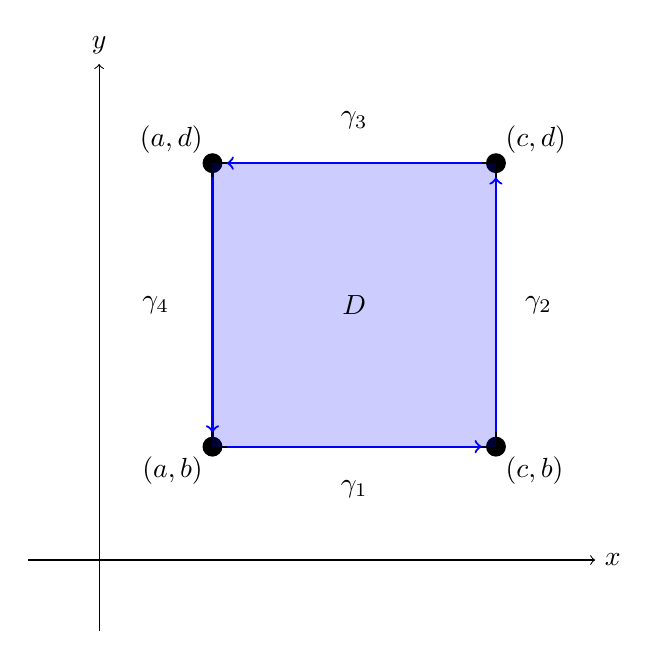
\begin{tikzpicture}[scale=1.8]
            % Ejes
            \draw[->] (-0.5, 0) -- (3.5, 0) node[right] {$x$};
            \draw[->] (0, -0.5) -- (0, 3.5) node[above] {$y$};

            % Rectángulo D
            \draw[thick, color=black] (0.8, 0.8) -- (2.8, 0.8) -- (2.8, 2.8) -- (0.8, 2.8) -- cycle;

            % Vértices
            \fill (0.8, 0.8) circle (2pt) node[below left] {$(a,b)$};
            \fill (2.8, 0.8) circle (2pt) node[below right] {$(c,b)$};
            \fill (2.8, 2.8) circle (2pt) node[above right] {$(c,d)$};
            \fill (0.8, 2.8) circle (2pt) node[above left] {$(a,d)$};

            % Región D
            \fill[opacity=0.2, color=blue] (0.8, 0.8) -- (2.8, 0.8) -- (2.8, 2.8) -- (0.8, 2.8) -- cycle;
            \node at (1.8, 1.8) {$D$};

            % Aristas con flechas y etiquetas
            \draw[thick, ->, color=blue] (0.9, 0.8) -- (2.7, 0.8);
            \node at (1.8, 0.5) {$\gamma_1$};

            \draw[thick, ->, color=blue] (2.8, 0.9) -- (2.8, 2.7);
            \node at (3.1, 1.8) {$\gamma_2$};

            \draw[thick, ->, color=blue] (2.7, 2.8) -- (0.9, 2.8);
            \node at (1.8, 3.1) {$\gamma_3$};

            \draw[thick, ->, color=blue] (0.8, 2.7) -- (0.8, 0.9);
            \node at (0.4, 1.8) {$\gamma_4$};
        \end{tikzpicture}
        \end{center}

        \textbf{Contribución de las aristas horizontales:}

        Para $\gamma_1$, parametrizamos como $\alpha_1(t) = (t, b)$ con $t \in [a,c]$, por lo que $d\alpha_1 = (dt, 0)$. Así:
        $$\oint_{\gamma_1} F = \int_a^c \langle (F_1(t,b), F_2(t,b)), (1, 0) \rangle dt = \int_a^c F_1(t, b) dt$$

        Para $\gamma_3$, parametrizamos como $\alpha_3(t) = (t, d)$ con $t \in [c,a]$ (orientación negativa), de modo que:
        $$\int_{\gamma_3} F \cdot d\gamma = \int_c^a F_1(t, d) dt = -\int_a^c F_1(t, d) dt$$

        La contribución total de las aristas horizontales es:
        $$\int_{\gamma_1 \cup \gamma_3} F_1 dx = \int_a^c [F_1(t, b) - F_1(t, d)] dt$$

        Por el Teorema Fundamental del Cálculo aplicado a la variable $y$:
        $$F_1(t, b) - F_1(t, d) = -\int_b^d \frac{\partial F_1}{\partial y}(t, y) dy$$

        En consecuencia:
        $$\int_{\gamma_1 \cup \gamma_3} F_1 dx = -\int_a^c \left(\int_b^d \frac{\partial F_1}{\partial y}(t, y) dy\right) dt$$

        \textbf{Contribución de las aristas verticales:}

        De forma análoga, para $\gamma_2$ (de $(c,b)$ a $(c,d)$) y $\gamma_4$ (de $(a,d)$ a $(a,b)$), obtenemos:
        $$\int_{\gamma_2 \cup \gamma_4} F_2 dy = \int_b^d \left(\int_a^c \frac{\partial F_2}{\partial x}(x, s) dx\right) ds$$

        \textbf{Conclusión:} Combinando ambas contribuciones:
        $$\oint_{\gamma} F \cdot d\gamma = \int_a^c \left(\int_b^d \frac{\partial F_2}{\partial x} - \frac{\partial F_1}{\partial y} dy\right) dx = \iint_D \left(\frac{\partial F_2}{\partial x} - \frac{\partial F_1}{\partial y}\right) dA$$

        por el Teorema de Fubini.
        \item \textbf{Caso 2:} Supongamos que $D$ es de la forma
        $$D = \{(x,y) : a \leq x \leq b, 0 \leq y \leq h(x)\}$$
        donde $h: [a,b] \to \mathbb{R}$ es una función diferenciable y positiva. Sea $S$ el rectángulo en $\mathbb{R}^2$ definido por 
        $$S = \{(x,y) : a \leq x \leq b, 0 \leq y \leq 1\}$$ y definimos $\varphi: S \to D$ por 
        $$\varphi(x,y) = (x, y h(x))$$
        Entonces $\varphi$ es biyectiva y diferenciable. Además, si $\alpha: [c,d] \to \mathbb{R}^2$ es una parametrización  de la frontera $\sigma$ del rectángulo $S$ orientada positivamente, entonces $\beta = \varphi \circ \alpha$ es una parametrización de $\gamma$ orientada positivamente. Así,
        $$\oint_{\gamma} F = \int_c^d \langle F(\beta(t)), \beta^{\prime}(t) \rangle dt = \int_c^d \langle F(\varphi(\alpha(t))), \varphi^{\prime}(\alpha(t)) \alpha^{\prime}(t) \rangle dt$$
        Por la transformación lineal $\varphi^{\prime}(x,y)$ tiene como matriz jacobiana
        $$\varphi^{\prime}(x, y) = \begin{pmatrix}
            1 & 0 \\
            yh^{\prime}(x) & h(x)
        \end{pmatrix}$$
        En particular $\varphi^{\prime}(x,y)$ es invertible por lo que $\varphi^{-1}$ es diferenciable. Además, por las propiedades del producto escalar tenemos que 
        $$\langle F(\varphi(\alpha(t)))\, \varphi^{\prime}(\alpha(t))\alpha^{\prime}(t) \rangle = \langle F(\varphi(\alpha(t))) \varphi^{\prime}(\alpha(t))^T, \alpha^{\prime}(t) \rangle$$
        
        Ahora defínese $g: \sigma \to \mathbb{R}^2$, $g = (g_1(x, y), g_2(x, y))$ por $g(x, y) = \varphi^{\prime}(x,y)^{T}(F \circ \varphi(x, y))$. De aquí se deduce que 
        $$\oint_{\gamma} F = \int_c^d \langle \varphi^{\prime}(\alpha(t))^T(F \circ \varphi(\alpha(t))), \alpha^{\prime}(t) \rangle dt = \int_c^d \langle g(\alpha(t)), \alpha^{\prime}(t) \rangle dt = \oint_{\sigma} g$$
        A partir de la expresión matricial de $\varphi^{\prime}(x,y)^T$ podemos calcular $g_1$ y $g_2$: 
        $$g_1(x,y) = F_1(x, yh(x)) + yh^{\prime}(x)F_2(x, yh(x))$$
        $$g_2(x,y) = h(x)F_2(x, yh(x))$$
        Por lo tanto, tenemos que 
        $$\frac{\partial g_1}{\partial y}(x,y) = h(x)\frac{\partial F_1}{\partial x}(x, yh(x)) + h^{\prime}(x) F_2(x, yh(x)) + yh^{\prime}(x)\frac{\partial F_2}{\partial y}(x, yh(x))h(x)$$
        $$\frac{\partial g_2}{\partial x}(x,y) = h^{\prime}(x)F_2(x, yh(x)) + h(x)\frac{\partial F_2}{\partial x}(x, yh(x)) + yh^{\prime}(x)\frac{\partial F_2}{\partial y}(x, yh(x))h(x)$$
        Ahora podemos aplicar el Caso 1: 
        $$\oint_{\sigma} g = \int_S (\frac{\partial g_2}{\partial x} - \frac{\partial g_1}{\partial y}) = \int_S \left(\frac{\partial F_2}{\partial x}(x, yh(x)) - \frac{\partial F_1}{\partial y}(x, yh(x))\right)h(x) = \int_S \left(\frac{\partial(F_2 \circ \varphi)}{\partial x} - \frac{\partial(F_1 \circ \varphi)}{\partial y}\right) |\varphi^{\prime}| =$$ $$ = \int_D \left(\frac{\partial F_2}{\partial x} - \frac{\partial F_1}{\partial y}\right) d\lambda_2$$
        \item \textbf{Caso 3:} Supongamos ahora que $\gamma$ es una curva cerrada orientada positivamente de clase $\mathcal{C}^1$ dada por $\alpha(t) = (\alpha_1(t), \alpha_2(t))$, $t \in [a,b]$. \\
        Podemos dividir la región $D$ en un número finito de regiones $D_1, D_2, \ldots, D_n$ en las condiciones de la proposición anterior (es decir, cada $D_i$ es de la forma del Caso 2), por lo que 
        $$\int_{\sigma_j} F = \int_{D_j} \left(\frac{\partial F_j}{\partial x} - \frac{\partial F_j}{\partial y}\right)$$
        donde $\sigma_j$ es una curva frontera del conjunto $D_j$. Como cada uno de los segmentos interiores horizontales o verticales aparece como frontera exactamente de las dos regiones, obsérvese que las contribuciones se cancelan: 
        $$\oint_{\gamma} F = \sum_{j = 1}^{m} \oint_{\sigma_j} F = \sum_{j = 1}^{m} \left(\frac{\partial F_2}{\partial x} - \frac{\partial F_1}{\partial y}\right) = \int_D \left(\frac{F_2}{\partial x} - \frac{\partial F_1}{\partial y}\right) d\lambda_2$$
        \item \textbf{Caso 4:} Sea $\gamma$ una curva cerrada, simple y rectificable parametrizada por una función absolutamente continua $u: [a, b] \to \mathbb{R}^2$ que encierra la región $D \subset \mathbb{R}^2$. Sea $\epsilon > 0$, por la densidad de $\mathcal{C}^1$ en $\mathcal{AC}$-funciones absolutamente continuas (Teorema de aproximación de Weierstrass), la continuidad de $F$ y la continuidad de la función área $A$, dado un $\delta > 0$ existe una curva $v \in \mathcal{C}^1([a, b], \mathbb{R}^2)$ que encierra la región $E$ tal que: 
        $$\|F \circ u - F \circ v\|_{\infty} \leq \delta, \quad \int_a^b \|u^{\prime} - v^{\prime}\| dt < \delta, \quad \lambda_2(D \Delta E) < \delta$$
        Tenemos entonces que 
        $$\left|\oint_u F - \oint_v F\right| = \left|\int_a^b \langle F(u(t)), u^{\prime}(t) \rangle - \langle F(v(t)), v^{\prime}(t) \rangle dt \right| = $$
        $$ = \left|\int_a^b \langle F(u(t)), u^{\prime}(t) \rangle - \langle F(v(t)), u^{\prime}(t)^\rangle + \langle F(v(t)), u^{\prime}(t)\rangle  - \langle F(v(t)), v^{\prime} \rangle dt \right| = $$
        $$ = \left|\int_a^b \rangle F(u(t)) - F(v(t)), u^{\prime}(t) \langle + \rangle F(v(t)), u^{\prime}(t) - v^{\prime}(t) \langle dt \right| = $$
        $$ \leq \int_a^b \|F(u(t)) - F(v(t))\| \|u^{\prime}(t) + \|F(v(t))\| \|u^{\prime}(t) - v^{\prime}(t)\| dt \leq$$
        $$ \leq 2\delta L(u) + \|F \circ v \|_{\infty} \delta \leq 2\delta L(u) + (\|F \circ u \|_{\infty} + \delta)\delta < \epsilon$$
        para $\delta$ lo suficientemente pequeño. \\
        Por otro lado: 
        $$\left|\int_D \left(\frac{\partial F_2}{\partial x} - \frac{\partial F_1}{\partial y}\right) - \int_E \left(\frac{\partial F_2}{\partial x} - \frac{\partial F_1}{\partial y}\right)\right| $$ $$\leq \int_{D \Delta E} \left|\frac{\partial F_2}{\partial x} - \frac{\partial F_1}{\partial y}\right| d\lambda_2 \leq \lambda_2(D \Delta E) \left\| \left(\frac{\partial F_2}{\partial x} - \frac{\partial{F_1}}{\partial y} \right) \Big|_{D \Delta E}  \right\|_{\infty} \leq \delta \left\|\left(\frac{\partial F_2}{\partial x} - \frac{\partial F_1}{\partial y}\right) \Big|_{D \Delta E}\right\|_{\infty} < \epsilon$$
        para $\delta$ suficientemente pequeño. Así, 
        $$- \epsilon + \oint_v F < \int_E \left(\frac{\partial F_2}{\partial x} - \frac{\partial F_1}{\partial y}\right) \leq \int_D \left(\frac{\partial F_2}{\partial x} - \frac{\partial F_1}{\partial y}\right) + \epsilon$$
        Como $\epsilon$ esta fijado arbitrariamente, tenemos que
        $$\oint_u F = \int_D \left(\frac{\partial F_2}{\partial x} - \frac{\partial F_1}{\partial y}\right)$$
    \end{enumerate}
\end{proof}
\begin{observación}
    Con el argumento de la densidad podemos reducir la regularidad de $F$ de $\mathcal{C}^1$ a $\mathcal{AC}$.
\end{observación}
\subsubsection{Teorema de Stokes}
TODO
\subsection{Teorema de la divergencia}
\begin{teorema}[Teorema de la divergencia]
    Sea $A \subset \mathbb{R}^n$ abierto, $V \subset A$ compacto y con una frontera $S$ tal que para una parametrización adeucada $\gamma: X \to \mathbb{R}^n$, $\gamma$ es continua, $N_{\gamma}$ está definida y no es nulo en casi todo punto, y $N_{\gamma} \in L^1(U, \mathbb{R}^n)$. Si $F \in \mathcal{AC}(A, \mathbb{R}^n)$ entonces
    $$\int_V div F = \oint_S F$$   
\end{teorema}
\begin{proof}
    Haremos la demostración para $n = 3$, pero para el caso general, sería de forma análoga.
    \begin{enumerate}
        \item \textbf{Parte 1:} Comenzamos estudiando el caso en el que: 
        \item $$V = \{(x, y, z) \in \mathbb{R}^3 : (x,y) \in [a,b] \times [c,d], 0\leq z \leq f(x, y)\}$$
        Comenzamos calculando la integral de la izquierda: 
        $$\int_V div(F) = \int_a^b \int_c^d \int_0^{f(x,y)} \left(\frac{\partial F_1}{\partial x} + \frac{\partial F_2}{\partial y} + \frac{\partial F_3}{\partial z}\right) dz dy dx = $$
        $$ = \int_c^d \int_a^b \int_0^{f(x,y)} \frac{\partial F_1}{\partial x} dz dy dx + \int_a^b \int_c^d \int_0^{f(x,y)} \frac{\partial F_2}{\partial y} dz dy dx + \int_a^b \int_c^d \int_0^{f(x,y)} \frac{\partial F_3}{\partial z} dz dy dx = I_1 + I_2 + I_3$$
        Veamos ahora cómo podemos calcular cada uno de los sumandos de la derecha: 
        \begin{itemize}
            \item \textbf{Primer sumando:} Dado un elemento $y \in [c,d]$, denotemos por: 
            $$\Omega_y = \{(x, z) \in \mathbb{R}^2 : x \in [a,b], 0 \leq z \leq f(x,y)\}$$
            Entonces, la frontera de $\Omega_y$ orientada positivamente dada por 
            $$\partial \Omega_y = \sigma_y^1 + \sigma_y^2 - \sigma_y^3 - \sigma_y^4$$
            donde
            $$\sigma_y^1: t \in [a, b] \to \sigma_y^1(t) = (t, y, 0)$$
            $$\sigma_y^2: t \in [0, f(b,y)] \to \sigma_y^2(t) = (b, y, t)$$
            $$\sigma_y^3: t \in [a, b] \to \sigma_y^3(t) = (t, y, f(t,y))$$
            $$\sigma_y^4: t \in [0, f(a,y)] \to \sigma_y^4(t) = (a, y, t)$$
            Dado el campo vectorial $G_y(x, z) = (0, F_1(x, y, z))$ por el Teorema de Green tenemos que 
            $$\int_a^b \int_0^{f(x,y)} \frac{\partial F_1}{\partial x} dz dx = \oint_{\partial \Omega_y} G_y = $$
            $$ = \int_a^b (0, f_1(t, y, 0)) \cdot (1, 0) dt + \int_0^{f(b, y)} (0, F_1(b, y, t)) \cdot (0,1) dt $$
            $$ - \int_a^b (0, F_1(t, y, f(t, y))) \cdot  \left(1, \frac{\partial f}{\partial x}(t, y)\right) dt - \int_0^{f(a, y)} (0, F_1(a, y, t)) \cdot (0,1) dt = $$
            $$ = \int_0^{f(b, y)} F_1(b, y, t) dt - \int_0^{f(a, y)} F_1(a, y, t) dt - \int_a^b F_1(t, y, f(t, y))\frac{\partial f}{\partial x}(t, y) dt$$
            \item \textbf{Seguno sumando:} Dado un elemento $x \in [a, b]$ denotemos por 
            $$\Omega_x = \{(y, z) \in \mathbb{R}^2 : y \in [c,d], 0 \leq z \leq f(x, y)\}$$
            Entones la frontera de $\Omega_x$ está orientada positivamente por 
            $$\partial \Omega_x
 = \sigma_x^1 + \sigma_x^2 - \sigma_x^3 - \sigma_x^4$$
            donde
            $$\sigma_x^1: t \in [c, d] \to \sigma_x^1(t) = (x, t, 0)$$
            $$\sigma_x^2: t \in [0, f(x,d)] \to \sigma_x^2(t) = (x, d, t)$$
            $$\sigma_x^3: t \in [c, d] \to \sigma_x^3(t) = (x, t, f(x,t))$$
            $$\sigma_x^4: t \in [0, f(x,c)] \to \sigma_x^4(t) = (x, c, t)$$
            Dado el campo vectorial $G_x(y, z) = (0, F_2(x, y, z))$ por el Teorema de Green tenemos que 
            $$\int_c^d \int_0^{f(x, y)} \frac{\partial F_2}{\partial y}(x, y, z) dz dy = \oint_{\partial \Omega_x} G_x = $$
            $$ = \int_0^{f(x, d)} F_d(x, d, t) dt - \int_0^{f(x, c)} F_2(x, c, t) dt - \int_c^d F_2(x, t, f(x, t)) \frac{\partial f}{\partial y}(x, t) dt$$
            \item \textbf{Tercer sumando: }
            $$ \int_a^b \int_c^d \int_0^{f(x, y)} \frac{\partial F_3}{\partial z} dz dy dx = \int_a^b \int_c^d [F_3(x, y, f(x, y)) - F_3(x, y, 0)] dy, dx$$
            Reagrupando los términos:
            $$\int_V div F = \int_c^d \int_0^{f(b, y)} F_1(b, y, t) dt dy - \int_c^d \int_0^{f(a, y)} F_1(a, y, t) dt dy - $$
            $$ - \int_c^d \int_a^b F_1(t, y, f(t, y)) \frac{\partial f}{\partial x}(t, y) dt dy + $$
            $$ + \int_a^b \int_0^{f(x, d)} F_2(x, d, t) dt dx - \int_a^b \int_0^{f(x, c) } F_2(x, c, t) dt dx - $$
            $$ - \int_a^b \int_c^d F_2(t, y, f(x, t))\frac{\partial f}{\partial y}(x, t) dt dx + $$
            $$ + \int_a^b \int_c^d F_3(x, y, f(x, y)) dy dx - \int_a^b \int_c^d F_3(x, y, 0) dy dx$$
            Se reordenan los sumandos: 
            $$\int_V div F = \int_c^d \int_0^{f(b, y)} F_1(b, y, z) dz dy - \int_c^d \int_0^{f(a, y)} F_1(a, y, z) dz dy + $$
            $$ + \int_a^b \int_0^{f(x, d)} F_2(x, d, z) dz dx - \int_a^b \int_0^{f(x, c)} F_2(x, c, z) dz dx - $$
            $$ - \int_a^b \int_c^d F_3(x, y, 0) dy dx - \int_a^b \int_c^d F_1(x, y, f(x, y)) \frac{\partial f}{\partial x}(x, y) dy dx - $$
            $$ - \int_a^b \int_c^d F_2(x, y, f(x, y)) \frac{\partial f}{\partial y} dy dx + \int_a^b \int_c^d F_3(x, y, f(x, y)) dy dx$$
            Calculemos ahora la integral de superficie. Denotemos por: 
            $$\partial \Omega_1 = \{(x, y, 0) : (x, y) \in [a,b] \times [c,d]\}$$
            $$\partial \Omega_2 = \{(x, y, f(x, y)) : (x, y) \in [a,b] \times [c,d]\}$$
            $$\partial \Omega_3 = \{(x, c, z) \in \mathbb{R}^3 : x \in [a,b], 0 \leq z \leq f(x, c)\}$$
            $$\partial \Omega_4 = \{(x, d, z) \in \mathbb{R}^3 : x \in [a, b], 0 \leq z \leq f(x, d)\}$$
            $$\partial \Omega_5 = \{(a, y, z) \in \mathbb{R}^3 : y  \in [c,d], 0 \leq z \leq f(a, y)\}$$
            $$\partial \Omega_6 = \{(b, y, z) \in \mathbb{R}^3 : y \in [c, d], 0 \leq z \leq f(b, y)\}$$
            Asociadas las parametrizaciones anteriores obtenemos los siguientes vectores normales: 
            $$N_1(x, y) 0 (0, 0, 1)$$
            $$N_2(x, y) = \left(-\frac{\partial f}{\partial x}, - \frac{\partial f}{\partial y}(x, y), 1\right)$$
            $$N_3(x, z) = (0, -1, 0)$$
            $$N_4(x, y) = (0, -1, 0)$$
            $$N_5(x,y) = (1, 0, 0)$$
            $$N_6(x, y) = (1, 0, 0)$$
            En vista de las orientaciones de los vectores normales tenemos que: 
            \begin{itemize}
                \item $N_1$ es nomral interior (hay que cambiar el signo)
                \item $N_2$ es normal exterior (se mantiene el signo)
                \item $N_3$ es normal exterior (se mantiene el signo)
                \item $N_4$ es normal interior (hay que cambiar el signo)
                \item $N_5$ es normal interior (hay que cambiar el signo)
                \item $N_6$ es normal exterior (se mantiene el signo)
            \end{itemize}
            Teniendo en cuenta la orientación de los vectores normales: 
            $$\oint_{\partial \Omega} F = - \oint_{\partial \Omega_1} F + \oint_{\partial \Omega_2} F + \oint_{\partial \Omega_3} F - \oint_{\partial \Omega_4} F - \oint_{\partial \Omega_5} F + \oint_{\partial \Omega_6} F$$
            Ahora, 
        \end{itemize}
    \end{enumerate}
\end{proof}